\documentclass[12pt,aspectratio=169]{beamer}

\usetheme[
    sectionpage=progressbar,
    subsectionpage=progressbar,
    progressbar=frametitle
]{metropolis}

\definecolor{blue-grey-900}{HTML}{263238}
\definecolor{deep-orange-500}{HTML}{FF5722}
\setbeamercolor{normal text}{fg=blue-grey-900, bg=white}
\setbeamercolor{alerted text}{fg=deep-orange-500}

\usepackage{booktabs}
\usepackage{graphicx}
\usepackage{hyphenat}
\usepackage{multirow}
\usepackage[normalem]{ulem}

\usepackage{polyglossia}
\setdefaultlanguage[variant=british]{english}
\usepackage[english=british]{csquotes}

\usepackage{fontspec}
\setmainfont{Lucida Sans OT}
\setsansfont[Scale=MatchLowercase]{Lucida Sans OT}
\setmonofont[Scale=MatchLowercase]{Lucida Console DK}
\defaultfontfeatures{Ligatures=TeX}

\usepackage{mathspec}
\setmathsfont(Digits,Latin,Greek)[Numbers={Lining,Proportional}]{Lucida Bright Math OT}

\renewcommand{\vec}[1]{\ensuremath{\mathbf{#1}}}
\newcommand{\mat}[1]{\ensuremath{\vec{#1}}}

\newcommand{\N}{\ensuremath{\mathbb{N}}}

\newcommand{\bshift}{\ensuremath{\mathcal{B}}}

\title{The Art of Forecasting}
\author{Gianluca Campanella}
\date{7\textsuperscript{th} June 2018}

\begin{document}

\maketitle

\begin{frame}{Hello!}
    \begin{center}
        \LARGE%
        My name is \textbf{Gianluca}
        {\fontspec{Gentium}\textcolor{gray}{[dʒanˈluːka]}}
    \end{center}
\end{frame}

\begin{frame}{What I do nowadays}
    \Large%
    \only<1>{%
        \begin{center}
            I'm a Data Scientist at \\[\bigskipamount]
            
\includegraphics[height=2.5em]{figures/microsoft} \\[\medskipamount]
            in \textbf{Algorithms and Data Science}
        \end{center}}
    \only<2>{%
        \begin{center}
            I also run my own company \\[\bigskipamount]
            \raisebox{-0.5\height}{
\includegraphics[height=2.5em]{figures/estimand}}
            \raisebox{-0.5\height}{\huge Estimand.com} \\[\medskipamount]
            that provides \\
            \textbf{Data Science training and mentoring}
        \end{center}}
\end{frame}

\begin{frame}{Today's slides}
    \centering\LARGE%
    \url{https://github.com/gcampanella/ndr-2018}
\end{frame}

\begin{frame}{References}
    \begin{center}
        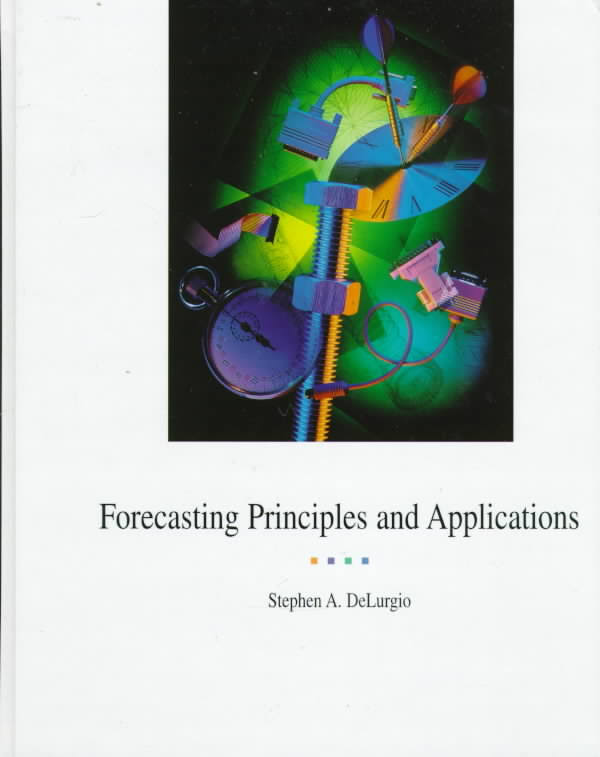
\includegraphics[height=0.8\textheight]{figures/delurgio}
        \hspace{2em}
        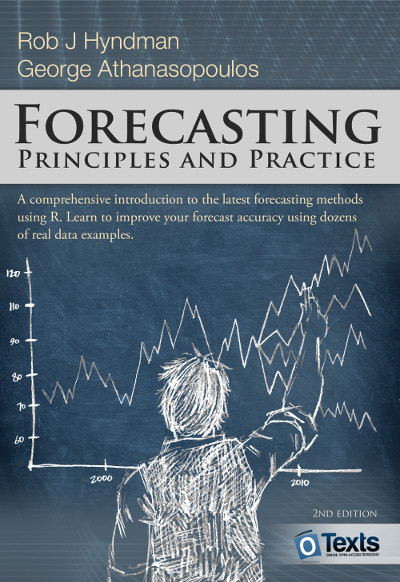
\includegraphics[height=0.8\textheight]{figures/fpp2}
    \end{center}
\end{frame}

\begin{frame}{Contents}
    \tableofcontents[hideallsubsections]
\end{frame}

\begin{frame}{What's a time series?}
    \begin{center}
        \Large%
        Any data that change \alert{over time}
    \end{center}
    \vfill
    \begin{itemize}
        \item Typically continuous (including counts)
        \item Time gives natural ordering
    \end{itemize}
\end{frame}

\begin{frame}{What's forecasting?}
    \begin{block}{Regression}
        \begin{itemize}
            \item Value of $\vec{y}$ given values for the predictors $\mat{X}$
            \item Does not depend on time (or temporal effect is negligible)
        \end{itemize}
    \end{block}
    \vfill\pause
    \begin{block}{Forecasting}
        \begin{itemize}
            \item Value of $\vec{y}$ given \alert{previous values} of $\vec{y}$
            \item Some models can also incorporate exogenous predictors
        \end{itemize}
    \end{block}
\end{frame}

\begin{frame}{Predictability}
    \only<1>{
        \begin{center}
            \Large%
            Can we forecast in changing environments?
        \end{center}}
    \only<2>{%
        Predictability depends on\ldots
        \begin{itemize}
            \item Availability of data
            \item Our understanding of contributing factors
            \item Whether our forecasts affect the process we're trying to
                  forecast
        \end{itemize}}
\end{frame}

\begin{frame}{A word of caution}
    \only<1>{%
        \begin{center}
            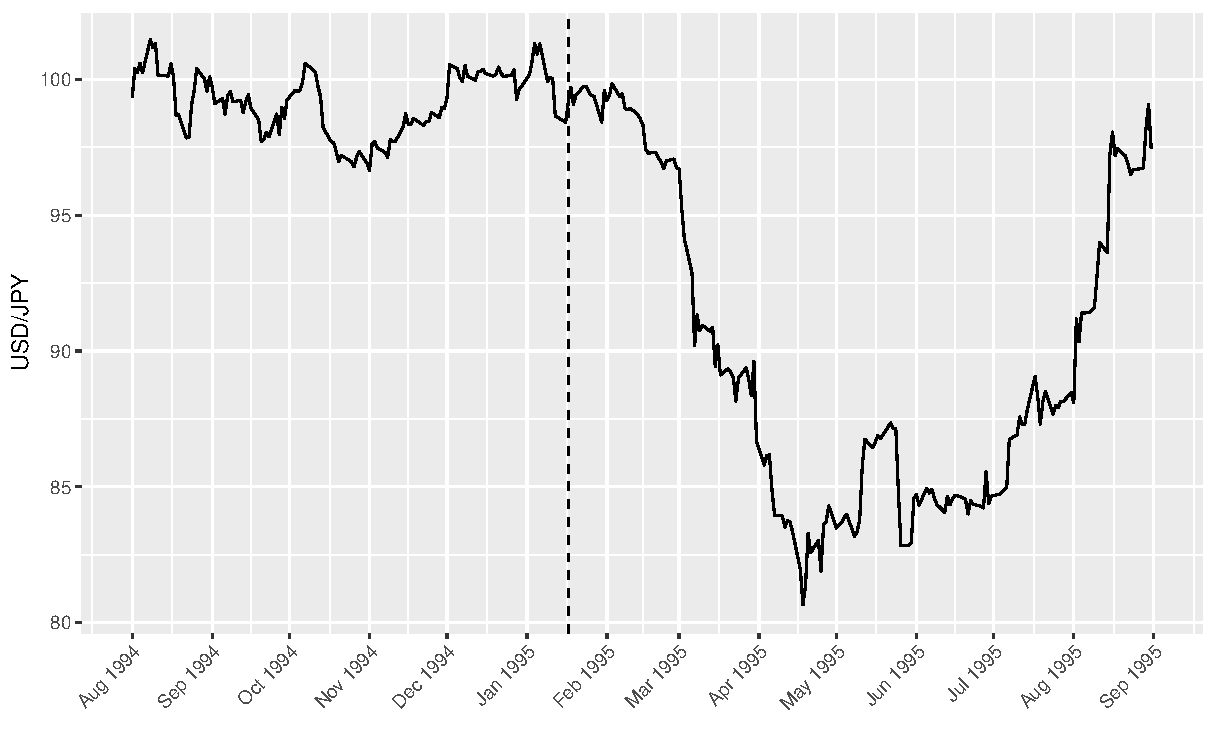
\includegraphics[height=0.8\textheight]{figures/usd_jpy}
        \end{center}}
    \only<2>{%
        \begin{center}
            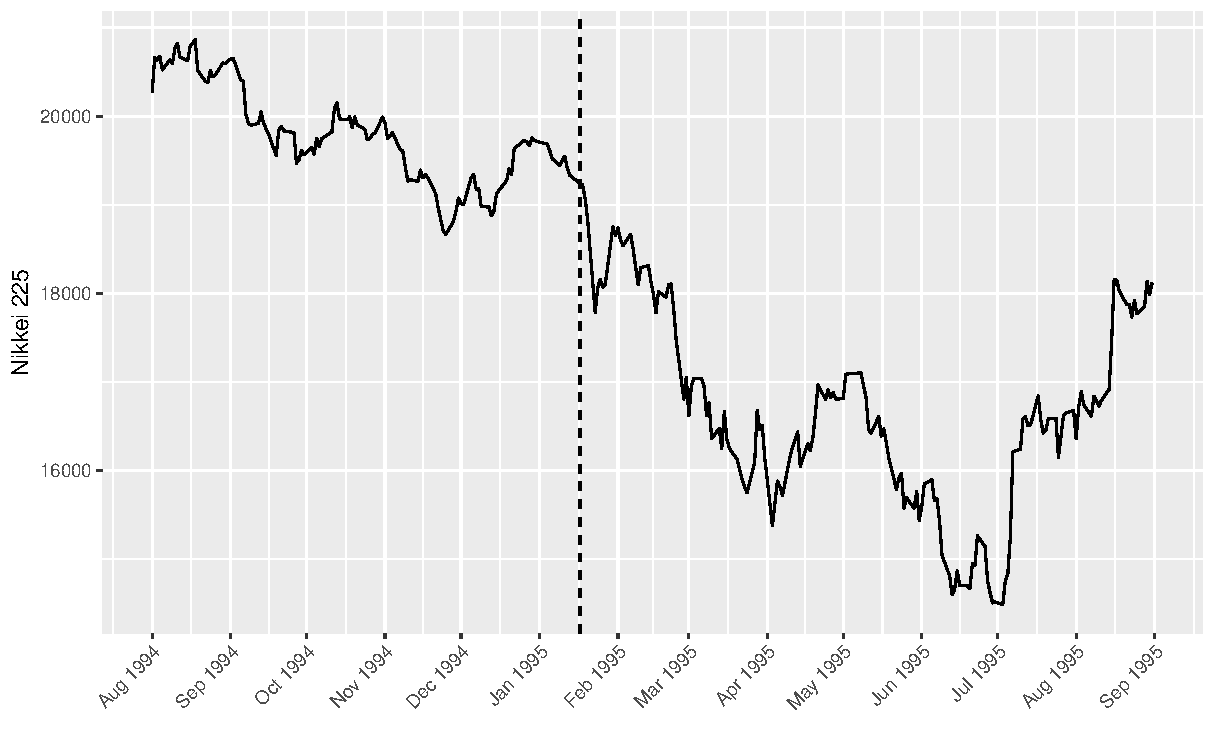
\includegraphics[height=0.8\textheight]{figures/nikkei_225}
        \end{center}}
    \only<3>{%
        \begin{center}
            \Large%
            What happened?
        \end{center}}
    \only<4>{%
        \begin{center}
            
\includegraphics[height=0.8\textheight]{figures/leeson_time_cover}
        \end{center}}
\end{frame}

\section{Motivation}

\begin{frame}{Motivation}
    \only<1>{%
        \begin{center}
            
\includegraphics[height=0.8\textheight]{figures/deaths_2015_avvenire}
        \end{center}}
    \only<2>{%
        \begin{center}
            
\includegraphics[height=0.8\textheight]{figures/deaths_2015_repubblica}
        \end{center}}
    \only<3>{%
        \begin{center}
            
\includegraphics[height=0.8\textheight]{figures/deaths_2015_sole}
        \end{center}}
    \only<4>{%
        \begin{columns}
            \begin{column}{0.6\textwidth}
                \begin{center}
                    \url{http://demo.istat.it/} \\[2em]
                    $\downarrow$ \\[2em]
                    \url{https://github.com/gcampanella/istat-demographics}
                \end{center}
            \end{column}
            \begin{column}{0.4\textwidth}
                \centering%
                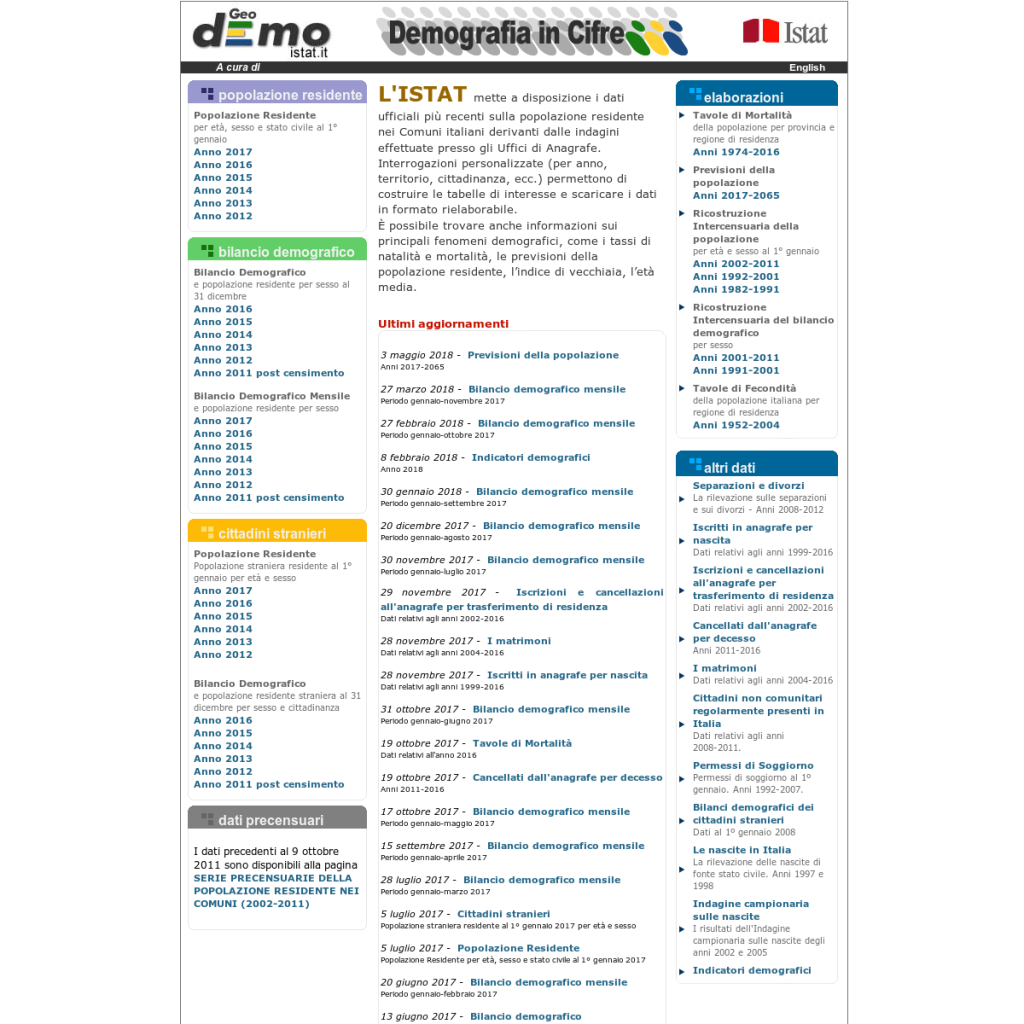
\includegraphics[height=0.8\textheight]{figures/demo_istat}
            \end{column}
        \end{columns}}
    \only<5>{%
        \begin{center}
            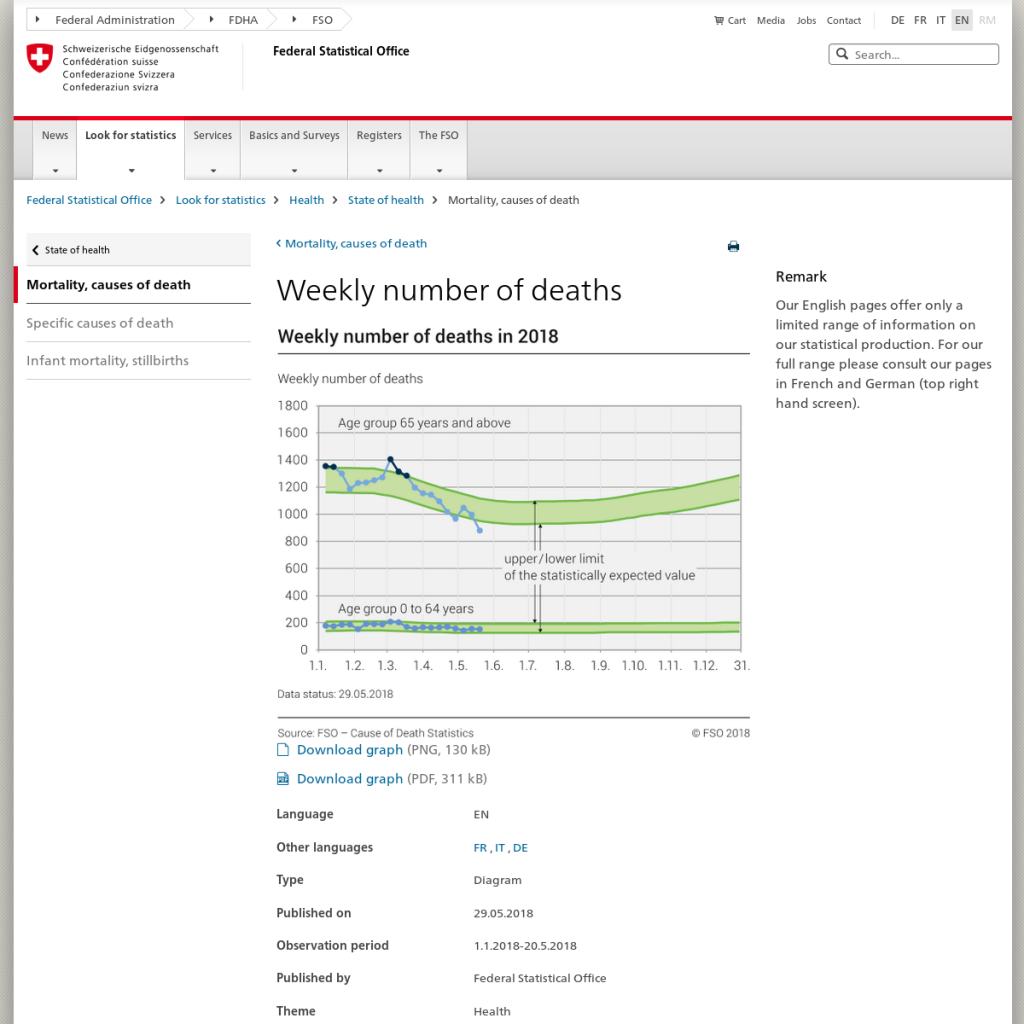
\includegraphics[height=0.8\textheight]{figures/fso}
        \end{center}}
\end{frame}

\begin{frame}{Data}
    \only<1>{%
        \begin{block}{Original data}
            \begin{itemize}
                \item Births, deaths, and net migration
                \item Monthly resolution from January 2004 till November 2017
                \item At municipality (\textit{comune}) level
                \item Stratified by sex
            \end{itemize}
        \end{block}}
    \only<2>{%
        \begin{block}{Aggregated data}
            \begin{itemize}
                \item Deaths only
                \item Monthly resolution from January 2004 till November 2017
                \item At \alert{region} level ($N = 20$)
                \item Stratified by sex
            \end{itemize}
        \end{block}}
\end{frame}

\begin{frame}{Pre-processing}
    \begin{center}
        \Large%
        Data are \alert{unnormalised} monthly counts
    \end{center}
    \vfill
    \begin{itemize}
        \item Boundary changes
        \item Population size (pre\hyp{}census vs post\hyp{}census)
        \item Calendar adjustment
    \end{itemize}
\end{frame}

\begin{frame}{Exploratory data analysis}
    \centering%
    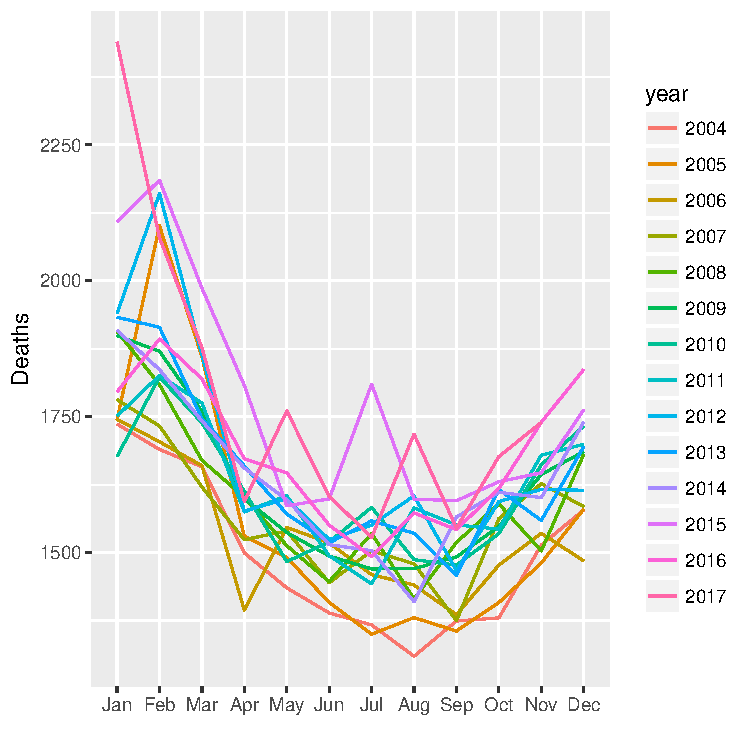
\includegraphics[height=0.8\textheight]{figures/total_deaths_by_month_and_year}
    \hspace{2em}
    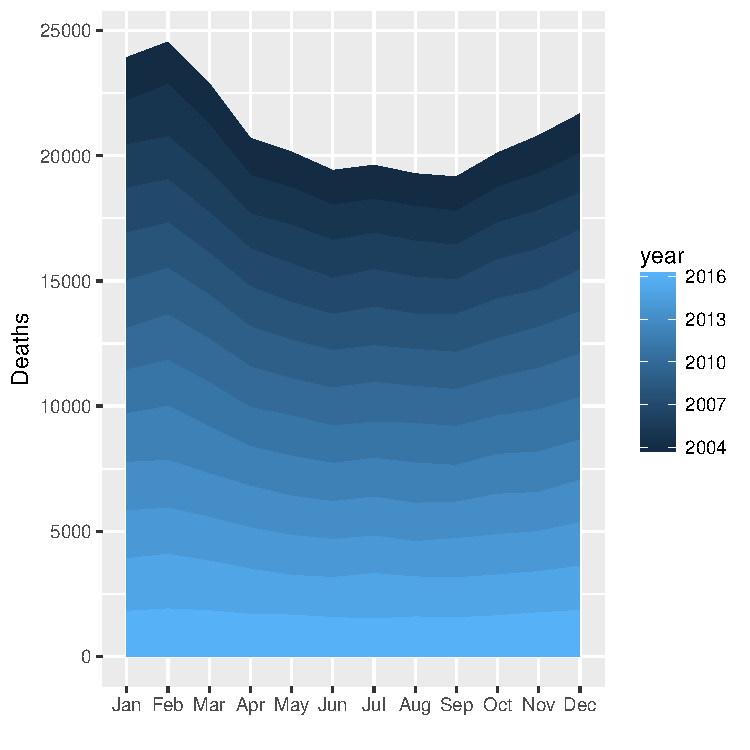
\includegraphics[height=0.8\textheight]{figures/total_cumulative_deaths_by_month}
\end{frame}

\begin{frame}{Analysis}
    \centering%
    \begin{tabular}{lll}
        \toprule
        \textbf{Family}               & \textbf{Method}  & \textbf{Package} \\
        \midrule
        \multirow{4}{*}{Baseline}     & Naïve (RW)       & \texttt{forecast} \\
                                      & Seasonal naïve   & \texttt{forecast} \\
                                      & Naïve with drift & \texttt{forecast} \\
                                      & Average          & \texttt{forecast} \\
        \midrule
        \multirow{4}{*}{Univariate}   & ETS              & \texttt{forecast} \\
                                      & ARIMA            & \texttt{forecast} \\
                                      & BSTS             & \texttt{bsts} \\
                                      & Prophet          & \texttt{prophet} \\
        \midrule
        \multirow{1}{*}{Hierarchical} & HTS              & \texttt{hts} \\
        \bottomrule
    \end{tabular}
\end{frame}

\section{Modelling}

\begin{frame}{Naïve and average methods}
    For all $h = 1, 2, \ldots$,
    \begin{center}
        \renewcommand{\arraystretch}{1.5}%
        \begin{tabular}{ll}
            \toprule
            \textbf{Naïve (RW)}                     & $\hat{y}_{T + h\,| T} = y_{T}$ \\
            \textbf{Seasonal naïve with period $m$} & $\hat{y}_{T + h\,| T} = y_{T+h-m(\lfloor (h-1)/m \rfloor+1)}$ \\
            \textbf{Naïve with drift}               & $\hat{y}_{T + h\,| T} = y_{T} + h\,(y_{t} - y_{1}) / (T - 1)$ \\
            \textbf{Average}                        & $\hat{y}_{T + h\,| T} = \sum_{t = 1}^{T} y_{t} / T$ \\
            \bottomrule
        \end{tabular}
    \end{center}
\end{frame}

\subsection{Exponential smoothing}

\begin{frame}{Simple exponential smoothing (SES)}
    Given a smoothing parameter $0 \leq \alpha \leq 1$,
    \[
        \hat{y}_{t + 1 | t} = \alpha y_{t} + (1 - \alpha) \hat{y}_{t\,| t - 1}
    \]
    \vfill
    \begin{align*}
        \hat{y}_{t + h | t} &= \ell_{t}                               & \text{(forecast)} \\
        \ell_{t}            &= \alpha y_{t} + (1 - \alpha) \ell_{t-1} & \text{(smoothing)}
    \end{align*}
\end{frame}

\begin{frame}{Holt's linear trend method}
    Given a smoothing parameter $0 \leq \beta \leq 1$,
    \begin{align*}
        \hat{y}_{t + h | t} &= \ell_{t} + \alert{h b_{t}}                                 & \text{(forecast)} \\
        \ell_{t}            &= \alpha y_{t} + (1 - \alpha) (\ell_{t-1} + \alert{b_{t-1}}) & \text{(level)} \\
        b_{t}               &= \beta (\ell_{t} - \ell_{t-1}) + (1 - \beta) b_{t-1}        & \text{(trend)}
    \end{align*}
\end{frame}

\begin{frame}{Gardner and McKenzie's damped trend method}
    Given a damping parameter $0 < \varphi < 1$,
    \begin{align*}
        \hat{y}_{t + h | t} &= \ell_{t} + \alert{(\varphi + \varphi^{2} + \ldots + \varphi^{h})} b_{t} & \text{(forecast)} \\
        \ell_{t}            &= \alpha y_{t} + (1 - \alpha) (\ell_{t-1} + \alert{\varphi} b_{t-1})      & \text{(level)} \\
        b_{t}               &= \beta (\ell_{t} - \ell_{t-1}) + (1 - \beta) \alert{\varphi} b_{t-1}     & \text{(trend)}
    \end{align*}
\end{frame}

\begin{frame}{Holt--Winters' seasonal (additive) method}
    Given a smoothing parameter $0 \leq \gamma \leq 1$ and a frequency $m \in \N$,
    \begin{align*}
        \hat{y}_{t + h | t} &= \ell_{t} + h b_{t} + \alert{s_{t+h-m(\lfloor (h-1)/m \rfloor+1)}}     & \text{(forecast)} \\
        \ell_{t}            &= \alpha (y_{t} - \alert{s_{t-m}} + (1 - \alpha) (\ell_{t-1} + b_{t-1}) & \text{(level)} \\
        b_{t}               &= \beta (\ell_{t} - \ell_{t-1}) + (1 - \beta) b_{t-1}                   & \text{(trend)} \\
        s_{t}               &= \gamma (y_{t} - \ell_{t}) + (1 - \gamma) s_{t-m}                      & \text{(seasonality)}
    \end{align*}
\end{frame}

\begin{frame}{ETS methods}
    \begin{columns}
        \begin{column}{0.475\textwidth}
            \begin{itemize}
                \item \alert{\textbf{E}rror}
                      \begin{itemize}
                          \item Additive
                          \item Multiplicative
                      \end{itemize}
                \item \textbf{T}rend
                      \begin{itemize}
                          \item None
                          \item Additive
                          \item Additive damped
                      \end{itemize}
                \item \textbf{S}easonality
                      \begin{itemize}
                          \item None
                          \item Additive
                          \item Multiplicative
                      \end{itemize}
            \end{itemize}
        \end{column}
        \begin{column}{0.05\textwidth}
            $\leadsto$
        \end{column}
        \begin{column}{0.475\textwidth}
            \centering%
            $2 \times 3 \times 3 = 18$ \\
            possible configurations
        \end{column}
    \end{columns}
\end{frame}

\subsection{ARIMA models}

\begin{frame}{Backshift operator $\bshift$}
    \only<1>{%
        Let's introduce the \alert{backshift operator $\bshift$},
        \begin{align*}
            \bshift y_{t}     &= y_{t-1} \\
            \bshift^{2} y_{t} &= y_{t-2} \\
                              &\vdots \\
            \bshift^{m} y_{t} &= y_{t-m}
        \end{align*}}
    \only<2>{%
        We can rewrite first\hyp{}order differences in terms of $\bshift$,
        \begin{align*}
            y_{t} - y_{t-1} &= y_{t} - \bshift y_{t} \\
                            &= (1 - \bshift) y_{t}
        \end{align*}
        \vfill\pause
        In general, $\bshift$ follows algebraic rules,
        \begin{align*}
            (1 - \bshift) (1 - \bshift^{m}) y_{t} &= (1 - \bshift^{m} - \bshift + \bshift^{m+1}) y_{t} \\
                                                  &= y_{t} - y_{t-m} - y_{t-1} + y_{t-m-1} \\
                                                  &= (y_{t} - y_{t-m}) - (y_{t-1} - y_{(t-1) - m})
        \end{align*}}
\end{frame}

\begin{frame}{Autoregressive and moving average models}
    \begin{block}{Autoregressive $\operatorname{AR}(p)$ model of order $p$}
        \[
            y_{t} = \beta_{0} + \beta_{1} y_{t-1} + \ldots + \beta_{p} y_{t-p} + \varepsilon_{t}
        \]
    \end{block}
    \vfill
    \begin{block}{Moving average $\operatorname{MA}(q)$ model of order $q$}
        \[
            y_{t} = \gamma_{0} + \gamma_{1} \varepsilon_{t-1} + \ldots + \gamma_{q} \varepsilon_{t-q} + \varepsilon_{t}
        \]
    \end{block}
\end{frame}

\begin{frame}{ARIMA models}
    \begin{block}{Non\hyp{}seasonal $\operatorname{ARIMA}(p, d, q)$ model}
        \[
            (1 - \beta_{1} \bshift - \ldots - \beta_{p} \bshift^{p}) (1 - \bshift)^{d} y_{t} = \alpha + (1 + \gamma_{1} \bshift + \ldots + \gamma_{q} \bshift^{q}) \varepsilon_{t}
        \]
    \end{block}
    \vfill\pause
    \begin{block}{Seasonal $\operatorname{ARIMA}(p, d, q)(P, D, Q)_{m}$ model}
        \vspace{-1em}
        \begin{align*}
            &(1 - \beta_{1} \bshift - \ldots - \beta_{p} \bshift^{p}) \alert{(1 - \Beta_{1} \bshift^{m} - \ldots - \Beta_{P} \bshift^{P m})} (1 - \bshift)^{d} \alert{(1 - \bshift^{D})} y_{t} \\
            &= \alpha + (1 + \gamma_{1} \bshift + \ldots + \gamma_{q} \bshift^{q}) \alert{(1 + \Gamma_{1} \bshift^{m} + \ldots + \Gamma_{Q} \bshift^{Q m})} \varepsilon_{t}
        \end{align*}
    \end{block}
\end{frame}

\subsection{Other methods}

\begin{frame}{Bayesian Structural Time Series (BSTS) models}
    \begin{itemize}
        \item Introduced by S.\ L.\ Scott and H.\ Varian (Google)
        \item Ensemble method
        \item Structural time series model + regression component
    \end{itemize}
    \vfill
    \begin{block}{Model evaluated}
        \begin{itemize}
            \item Local linear trend
            \item Seasonal model with $m = 12$
        \end{itemize}
    \end{block}
\end{frame}

\begin{frame}{Prophet}
    \begin{itemize}
        \item Introduced by S.\ J.\ Taylor​​ and B.\ Letham​ (Facebook)
        \item Curve fitting (similarly to GAMs)
        \item Decomposition into trend, seasonality, and holidays
    \end{itemize}
    \vfill
    \begin{block}{Model evaluated}
        \begin{itemize}
            \item Default settings
            \item[$\rightarrow$] No daily or weekly seasonality
        \end{itemize}
    \end{block}
\end{frame}

\begin{frame}{Hierarchical time series models}
    \begin{itemize}
        \item Introduced by R.\ J.\ Hyndman et al.\ (Monash University)
        \item Independent forecasts + aggregation at different levels
        \item Many different aggregation methods
    \end{itemize}
    \vfill
    \begin{block}{Models evaluated}
        \begin{itemize}
            \item Forecasting methods: ARIMA, ETS, RW
            \item 5 aggregation methods $\times$ 4 weighting schemes
        \end{itemize}
    \end{block}
\end{frame}

\subsection{Measures}

\begin{frame}{Scale-dependent measures}
    Given the prediction errors $e_{T + h} = y_{T + h} - \hat{y}_{T + h}$, \ldots
    \begin{center}
        \renewcommand{\arraystretch}{1.5}%
        \begin{tabular}{ll}
            \toprule
            \textbf{Measure} & \\
            \midrule
            \textbf{Mean absolute error}              & $\operatorname{mean}(|e_{t}|)$ \\
            \textbf{Root\hyp{}mean\hyp{}square error} & $\sqrt{\operatorname{mean}(e_{t}^{2})}$ \\
            \bottomrule
        \end{tabular}
    \end{center}
\end{frame}

\begin{frame}{Percentage errors}
    Given the \alert{percentage} errors $p_{t} = 100 e_{t} / y_{t}$, \ldots
    \begin{center}
        \renewcommand{\arraystretch}{1.5}%
        \begin{tabular}{ll}
            \toprule
            \textbf{Measure} & \\
            \midrule
            \textbf{Mean absolute percentage error} & $\operatorname{mean}(|p_{t}|)$ \\
            \textbf{Symmetric MAPE}                 & $\operatorname{mean}(200 |y_{t} - \hat{y}_{t}| / (y_{t} + \hat{y}_{t}))$ \\
            \bottomrule
        \end{tabular}
    \end{center}
\end{frame}

\begin{frame}{Scaled errors}
    Given the \alert{scaled} errors\ldots
    \[
        q_{t} = \frac{e_{t}}{\frac{1}{T-1} \sum_{t^{\prime} = 2}^{T} |y_{t^{\prime}} - y_{t^{\prime}-1}|}
        \qquad
        \text{or}
        \qquad
        q_{t} = \frac{e_{t}}{\frac{1}{T-m} \sum_{t^{\prime} = m+1}^{T} |y_{t^{\prime}} - y_{t^{\prime}-m}|}
        \text{,}
    \]
    the \textbf{mean absolute scaled error} is simply
    $\operatorname{mean}(|q_{t}|)$
    \vfill
    \begin{block}{Interpretation}
        For $q_{t} < 1$, the forecast is better than the average (seasonal)
        naïve forecast (computed on the training data)
    \end{block}
\end{frame}

\section{Results and recommendations}

\begin{frame}{Seasonal naïve forecasts}
    \centering%
    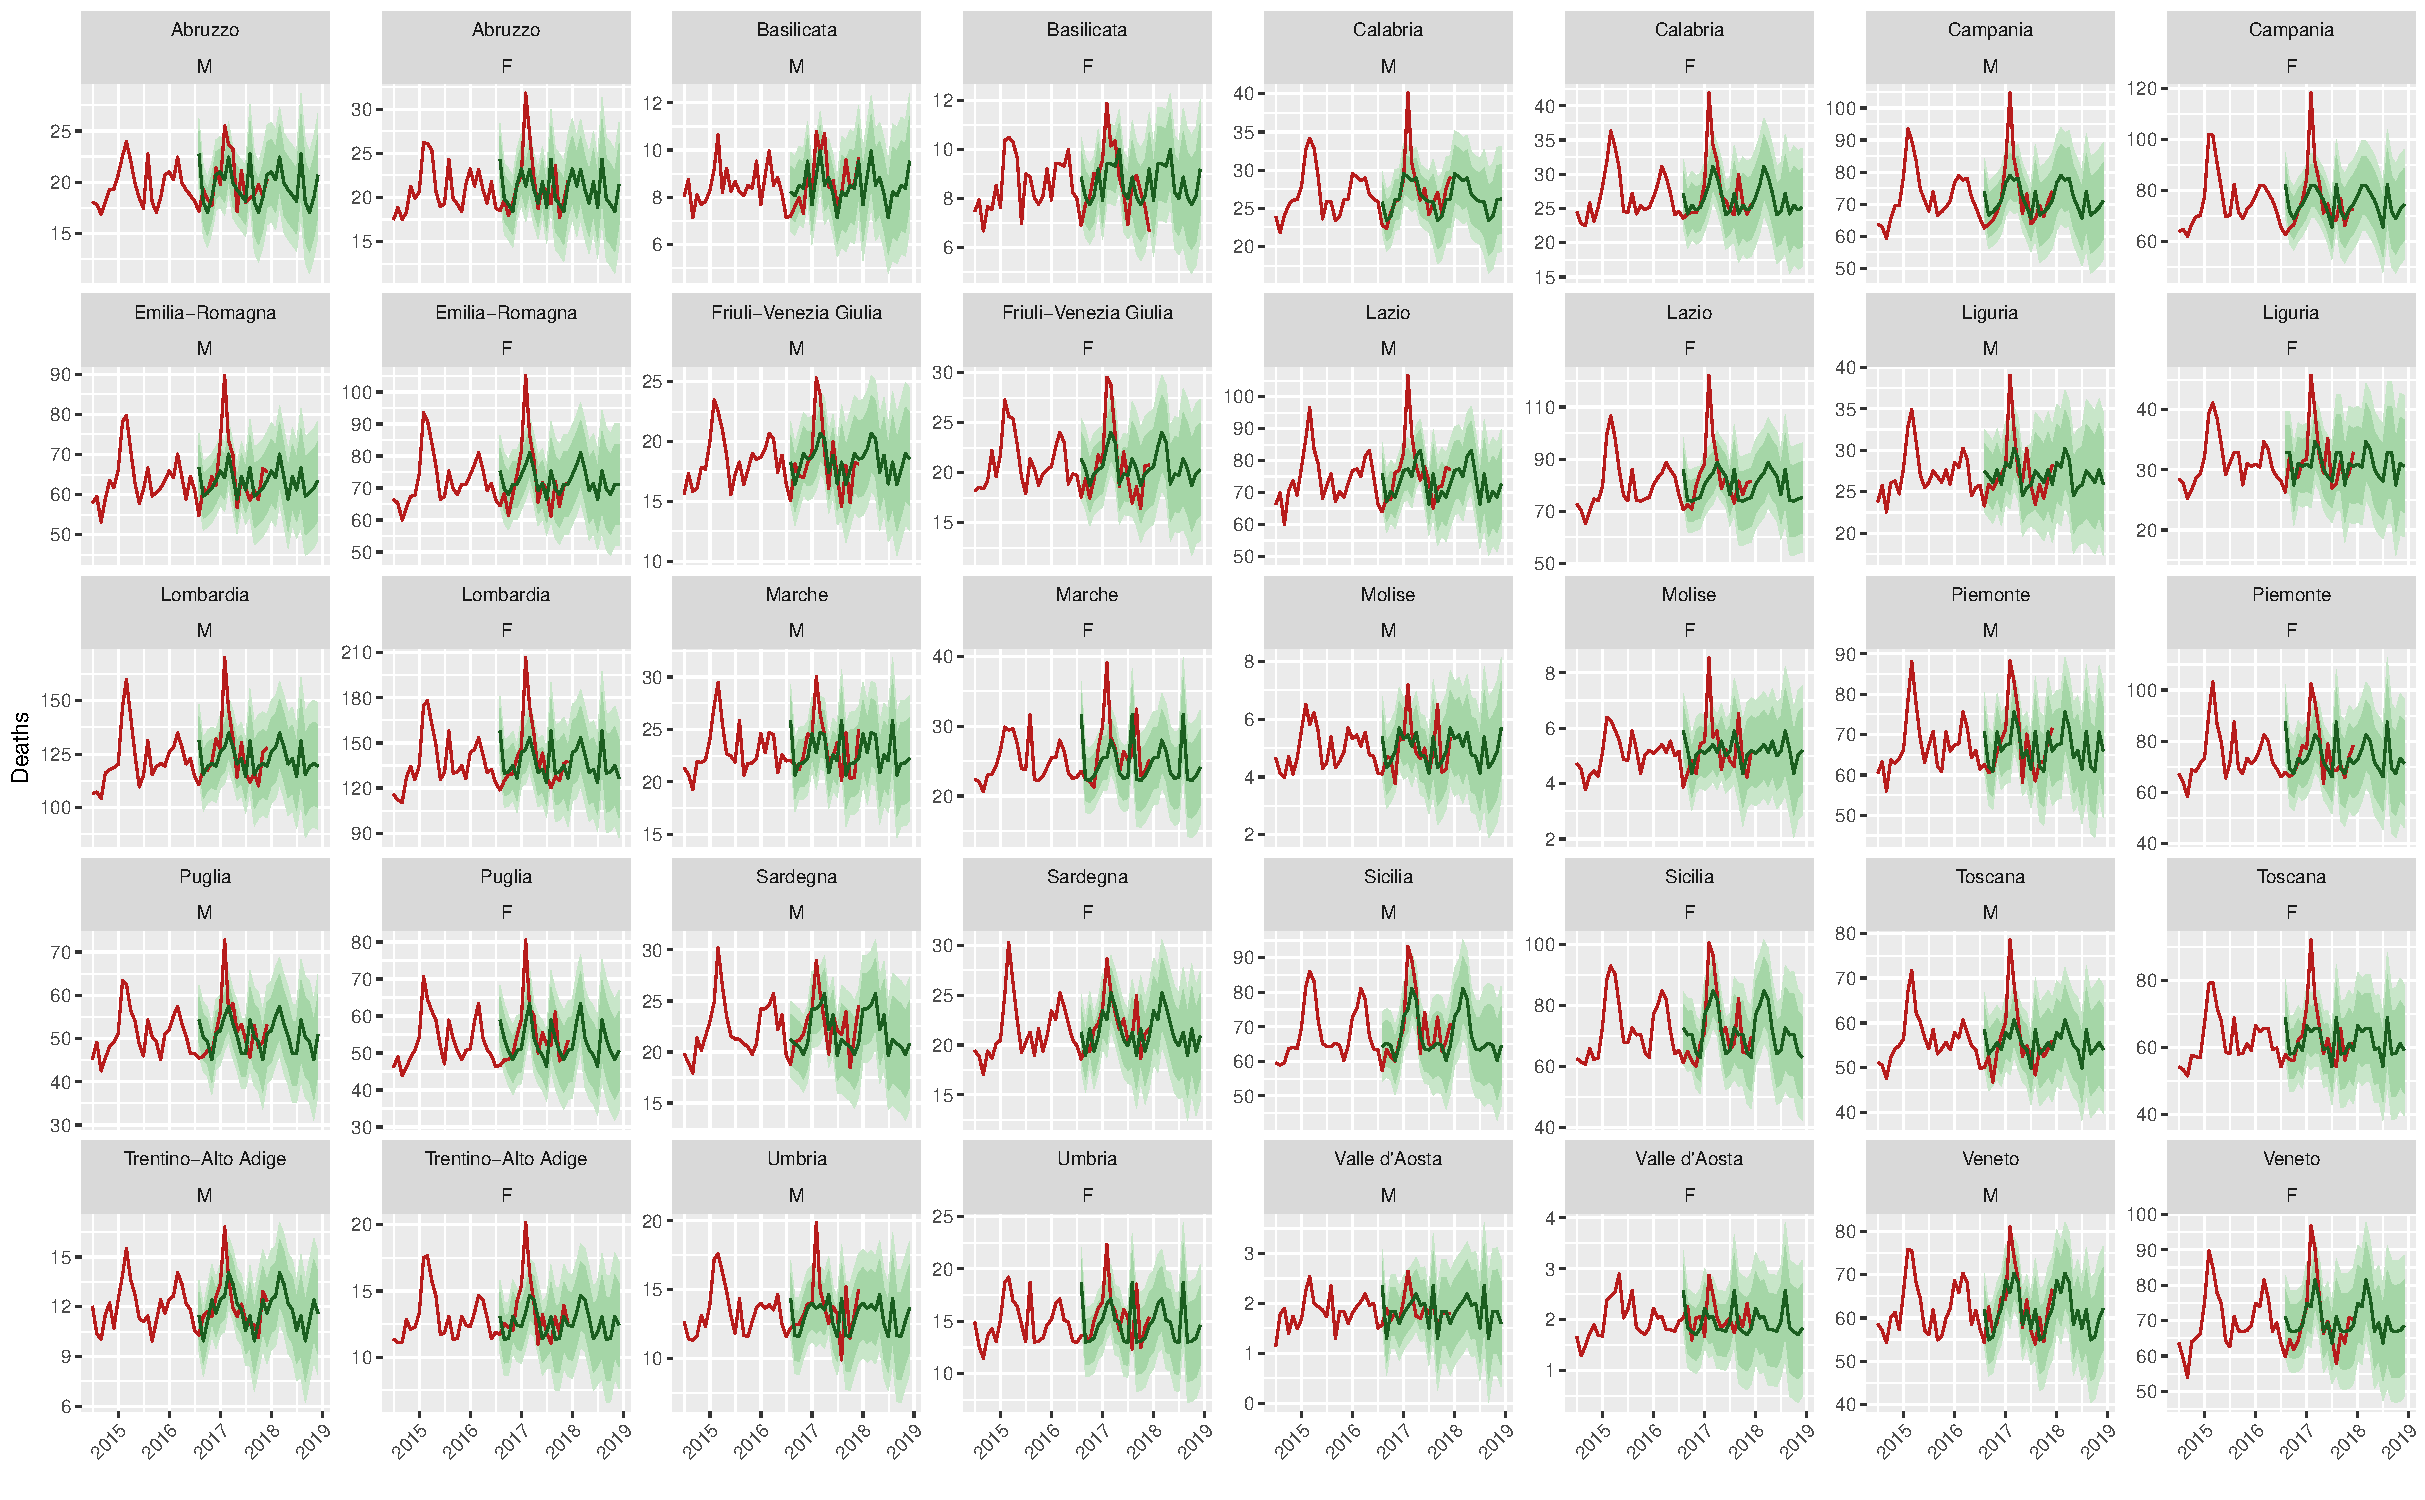
\includegraphics[height=0.9\textheight]{figures/forecasts_snaive}
\end{frame}

\begin{frame}{ETS forecasts}
    \centering%
    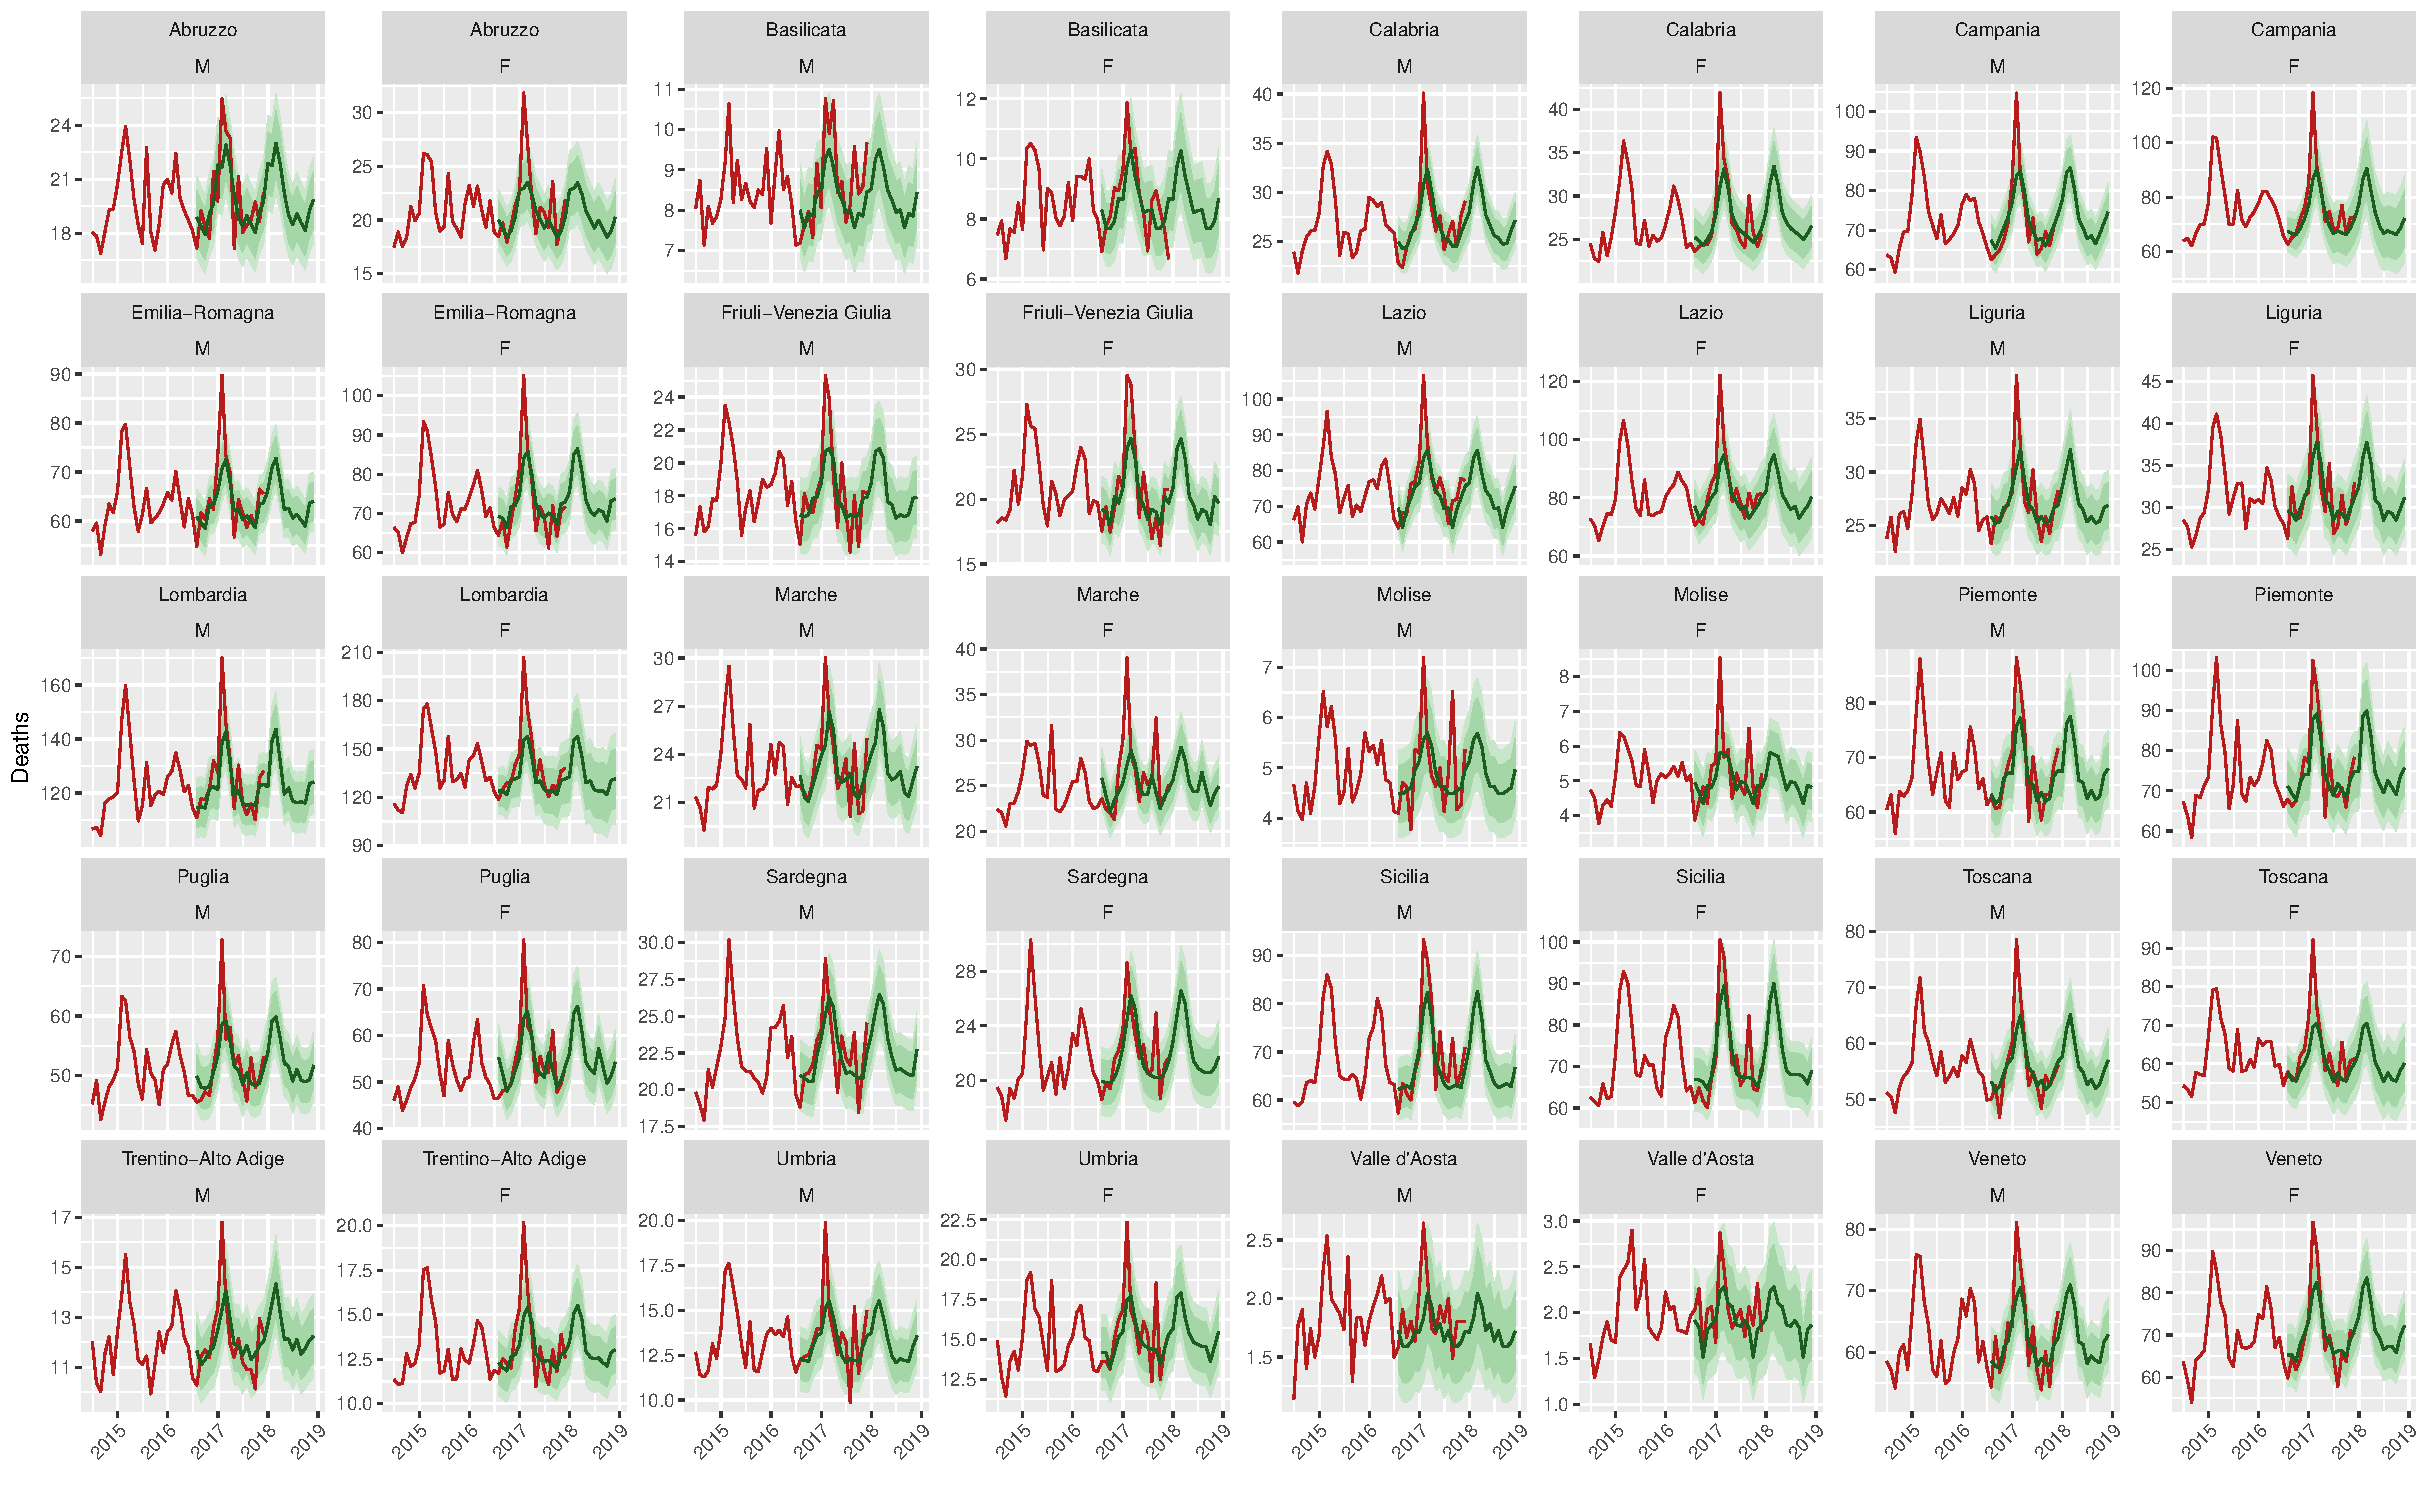
\includegraphics[height=0.9\textheight]{figures/forecasts_ets}
\end{frame}

\begin{frame}{Univariate models}
    \centering%
    \only<1>{%
        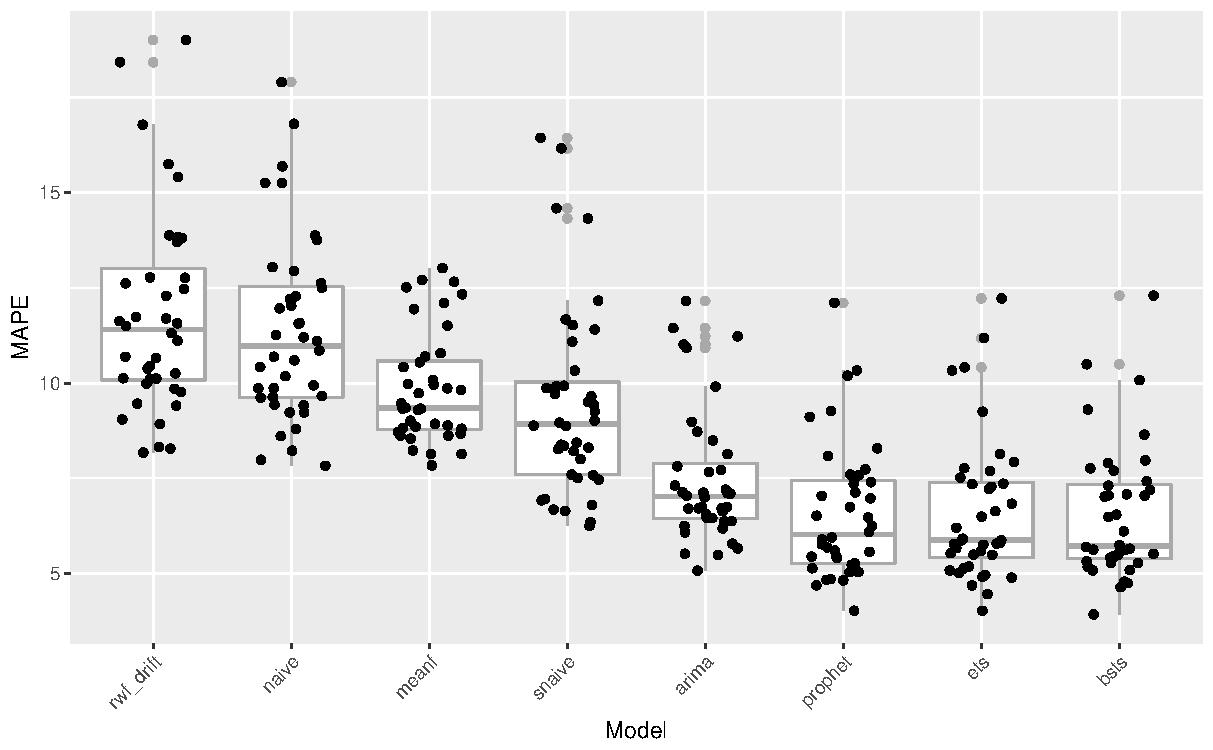
\includegraphics[height=0.9\textheight]{figures/mape_by_model}}
    \only<2>{%
        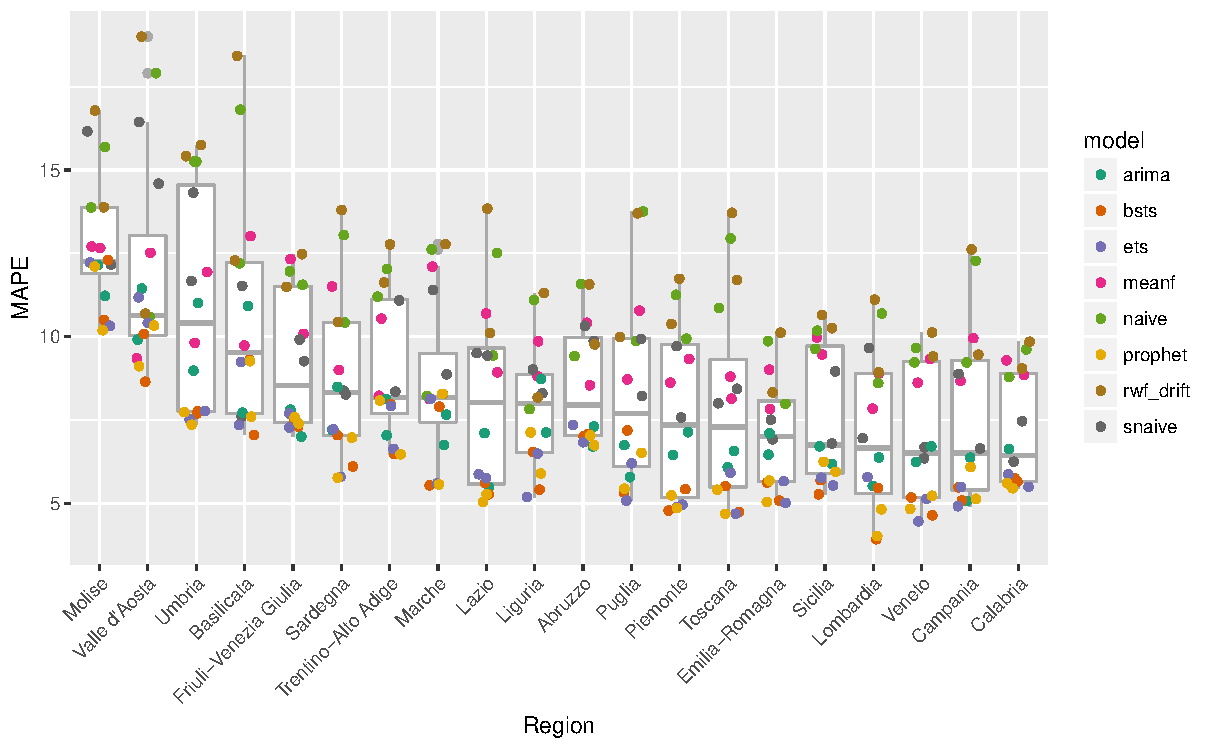
\includegraphics[height=0.9\textheight]{figures/mape_by_region}}
\end{frame}

\begin{frame}{HTS models}
    \centering%
    \only<1>{%
        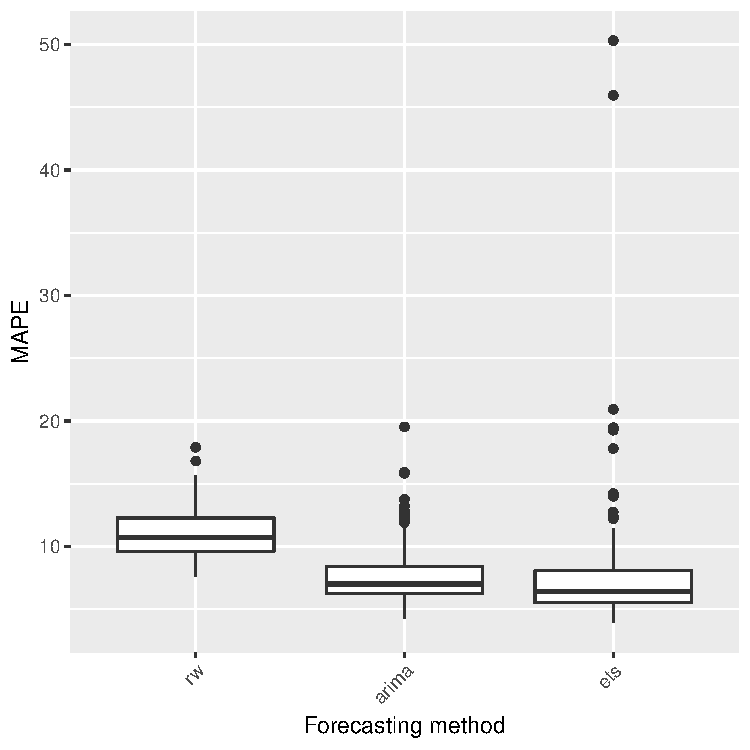
\includegraphics[height=0.8\textheight]{figures/hts_mape_by_fmethod}
        \hspace{2em}
        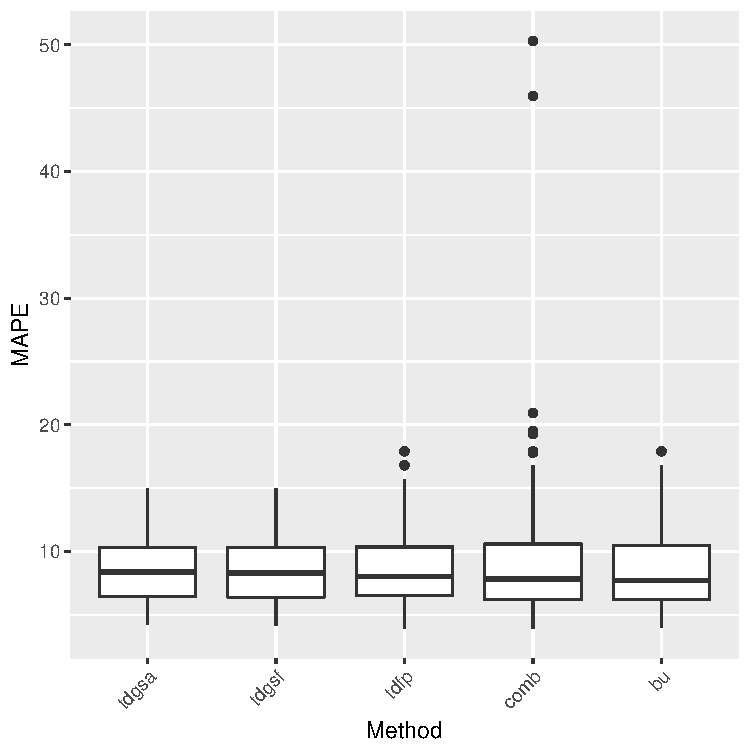
\includegraphics[height=0.8\textheight]{figures/hts_mape_by_method}}
    \only<2>{%
        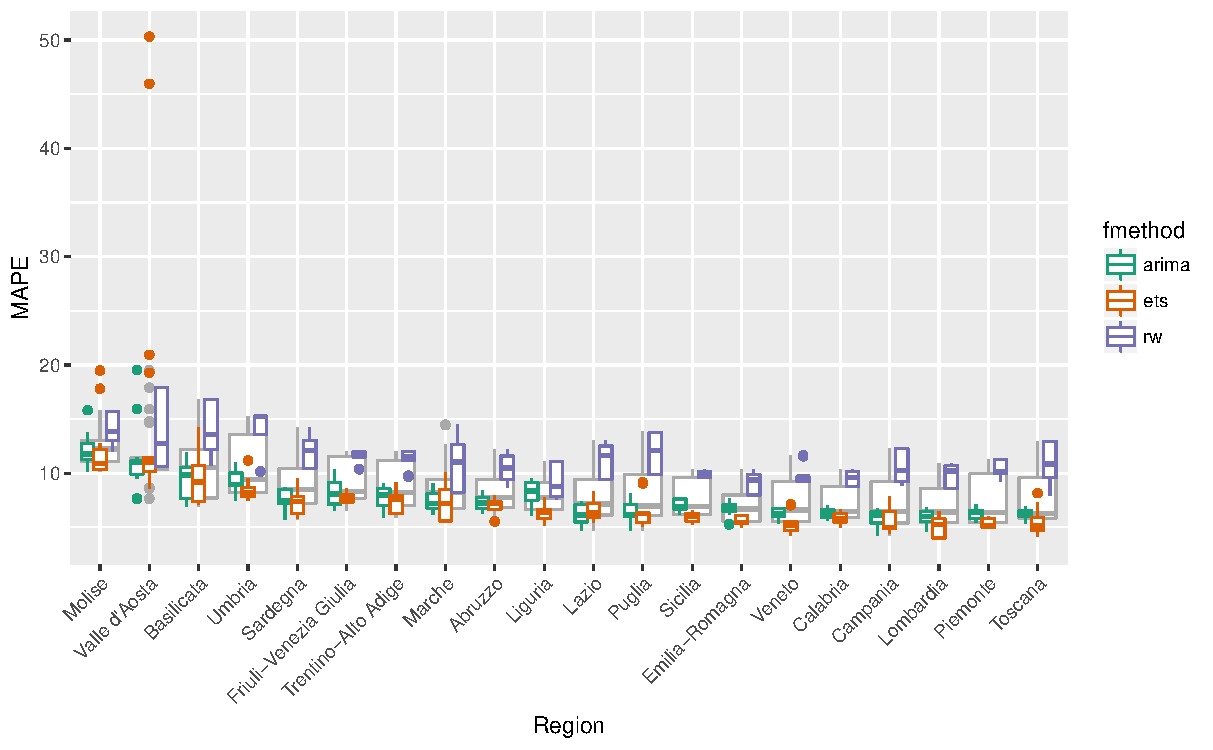
\includegraphics[height=0.9\textheight]{figures/hts_mape_by_region}}
\end{frame}

\begin{frame}{And the winner is\ldots}
    \centering%
    \begin{tabular}{lr}
        \toprule
        \textbf{Method} & \textbf{MAPE} \\
        \midrule
        BSTS                     & 6.52\% \\
        Prophet                  & 6.58\% \\
        ETS                      & 6.62\% \\
        HTS (bottom\hyp{}up ETS) & 6.62\% \\
        ARIMA                    & 7.49\% \\
        Seasonal naïve           & 9.44\% \\
        Average                  & 9.83\% \\
        Naïve (RW)               & 11.4\% \\
        Naïve with drift         & 11.8\% \\
        \bottomrule
    \end{tabular}
\end{frame}

\begin{frame}{Lessons learned}
    \only<1>{%
        \begin{block}{Time series are messy!}
            \begin{itemize}
                \item Temporal resolution and spacing
                \item Calendar adjustment
                \item Model evaluation and cross\hyp{}validation
                \item Hierarchical structure
            \end{itemize}
        \end{block}}
    \only<2>{%
        \begin{block}{Time series are fun!}
            \begin{itemize}
                \item Data visualisation
                \item Models (often) interpretable
                \item Anomaly detection
            \end{itemize}
        \end{block}}
\end{frame}

\begin{frame}{Future work}
    \begin{itemize}
        \setlength{\itemsep}{1em}
        \item Compare even more models (including neural networks)
        \item Include exogenous covariates such as temperature
        \item Build a user interface
    \end{itemize}
\end{frame}

\end{document}

